\chapter{Background}

% \section{Rendering an Image of a 3D Scene}
\section{Rendering}

This section gives an overview of rendering an image of a 3D scene to connect the image-level appearance with a broader concept of appearance representations in computer graphics.  It starts with the display of images on a screen and elaborates on 3D scene components that are taken into account for photorealistic rendering, mainly focusing on appearance. 

\subsection{Displaying an image}
An image is displayed on a computer screen or, in general, a display system, after the processing of the stored data in a computer. Here, both the computer and display system operate with discrete data, known as bits and pixels. Considering real-world objects as continuous structures, the object shapes need to be broken down into discrete surfaces, pixels, for the display of their image. This operation is known as discretization. 

Let's consider the display of a sphere on a computer screen. We apply a grid on the sphere to represent pixels. Some pixels have a constant color of the object, while some are blank. On the other hand, some pixels include different shades of the object color or some are half-overlapped with the sphere. The question here is how to fill the pixels with mixed colors. 


\begin{figure}
  \centering
  % \fbox{\rule{0pt}{2in} \rule{0.9\linewidth}{0pt}}

    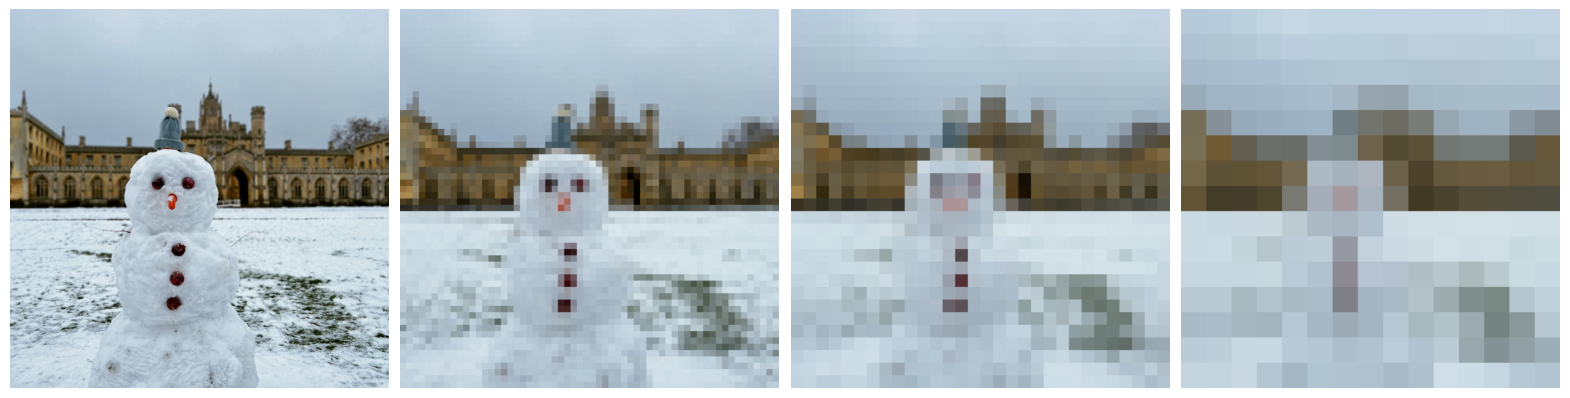
\includegraphics[width=\linewidth]{Images/pixelate_image_snowman.png}

   \caption{A pixel, picture element, is the smallest unit of a rendered image. Displaying an image with fewer pixels causes losses in details as one pixel starts covering a larger area in the 3D scene.}
   \label{fig:color-approximate}
\end{figure}


In a simple case where we only have a single color with a blank background, we can subdivide this pixel into sub-pixels and count the number of pixels that belong to the object and the background. Later, the color of the corresponding pixel can be approximated by taking the weighted average between the background and object color. For instance, Figure \ref{fig:display-grid} shows the display of a sphere with grids symbolizing pixels. The sub-pixels on the right can be counted to compute the color of the corresponding large pixel. The generalized implementation of this approach can be seen in Figure \ref{fig:color-approximate}, where I computed the mean value with a sliding window of different sizes (50, 100 and 200 in order for image size of 3024 x 4032).


\begin{figure}
  \centering
  % \fbox{\rule{0pt}{2in} \rule{0.9\linewidth}{0pt}}
   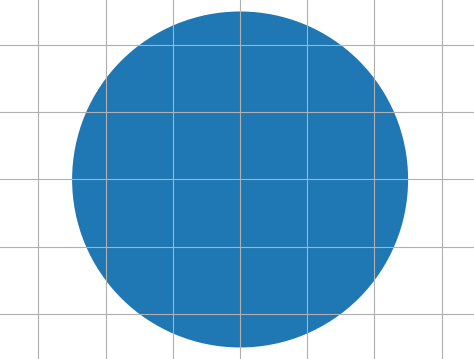
\includegraphics[width=0.4\linewidth]{Images/grid_circle.png}
    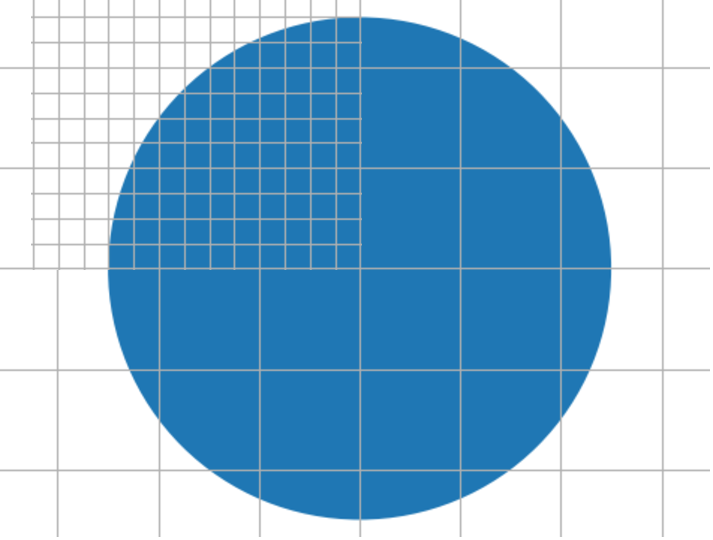
\includegraphics[width=0.4\linewidth]{Images/merged_grid_circle2-crop.pdf}

   \caption{Need a figure to represent pixel representation of continuous image}
   \label{fig:display-grid}
\end{figure}


\begin{wrapfigure}{l}{8.5cm}
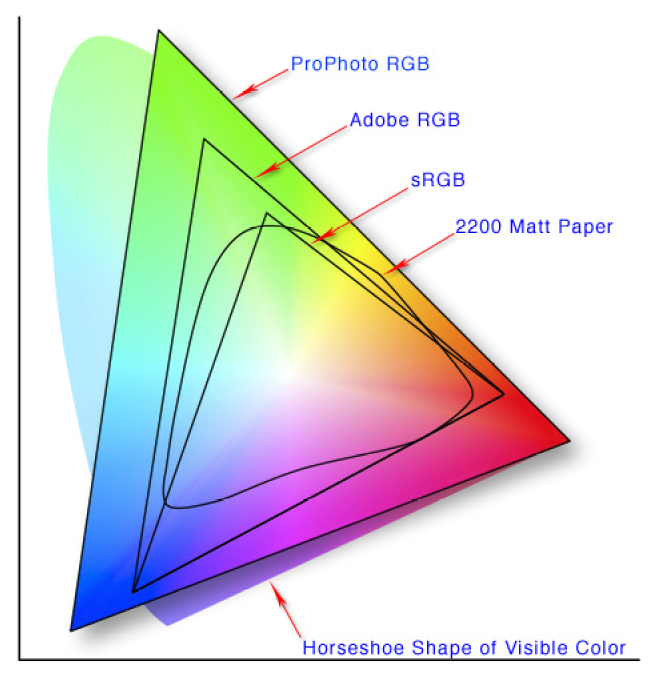
\includegraphics[width=0.9\linewidth]{Images/Colorspace.png}
\caption{Comparison of different color gamuts \cite{schewe2007color}}\label{fig:color-gamut}
    
\end{wrapfigure} 

Another approach would be to increase the resolution of an image, that is, increase the number of pixels per image. However, we will still be limited by the resolution of the screen. As we simulate the real world, the discretization process will remain a part of this virtual representation. It is also not only the surface of the objects we need discretize. The color of a pixel should also be broken down into pieces, bits, for the storage in computers. In other words, the number of colors that we can display is limited by the number of bits used to encode the color. 

When computers were first invented, the brightness of each pixel on the screen was encoded using just one bit. The pixel would be white when the bit value was 1, and black when it had a value of 0. These days, one of the most commonly used color spaces, standard RGB space (sRGB), encodes each color with 8 bits, requiring $8 * 3 = 24$ bits per pixel. Here, the question would be how to display a color that is not available in a color space. This problem is known as color quantization. The solution would be again approximating the desired color with the closest matching color available in the space/palette.

% \begin{figure}
%   \centering
% \caption{Comparison of different color gamuts \cite{schewe2007color}}\label{fig:color-gamut}
%     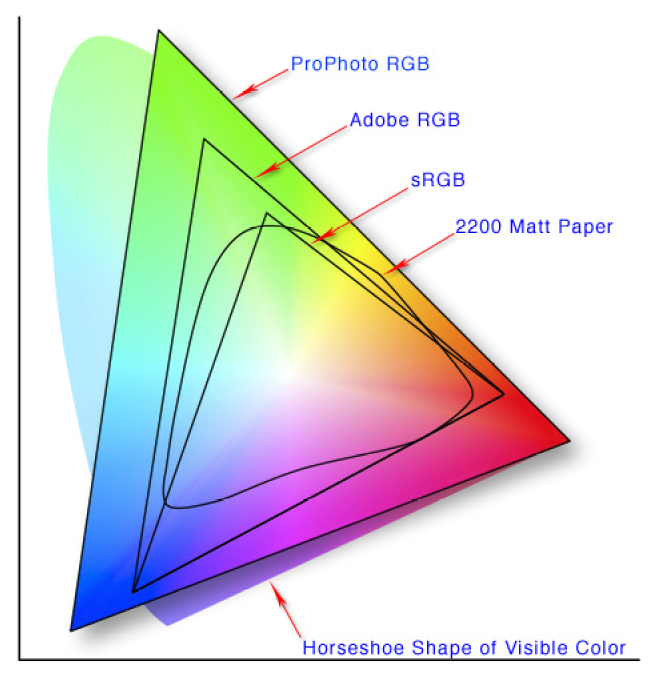
\includegraphics[width=0.44\linewidth]{Images/Colorspace.png}
% \end{figure} 
% %-----------------



The issue with color quantization is that few color samples might not accurately represent the continuous color spectrum, causing discrete steps, bands, between the color samples that can be visible in the images (Figure \ref{fig:color-band}). Luckily, the current image formats allow 24 (sRGB) / 32 (RGBA) bits to encode colors, displaying more than 16 million distinct colors, reducing the color banding effect significantly. Nevertheless, the representation of continuous signals in the virtual environment remains limited due to the discretization of the data with bits for the storage in a computer.

Another problem we need to consider is aliasing, which occurs when sampling frequency for discretization is lower than twice the continuous signal bandwidth (Nyquist Theorem). The range of frequencies you can capture in a scene depends on the image resolution or pixel size. For instance, if an object is too far, then its projection can be smaller than the pixel size, in which case we end up seeing the object as a dot.



\begin{figure}
  \centering
    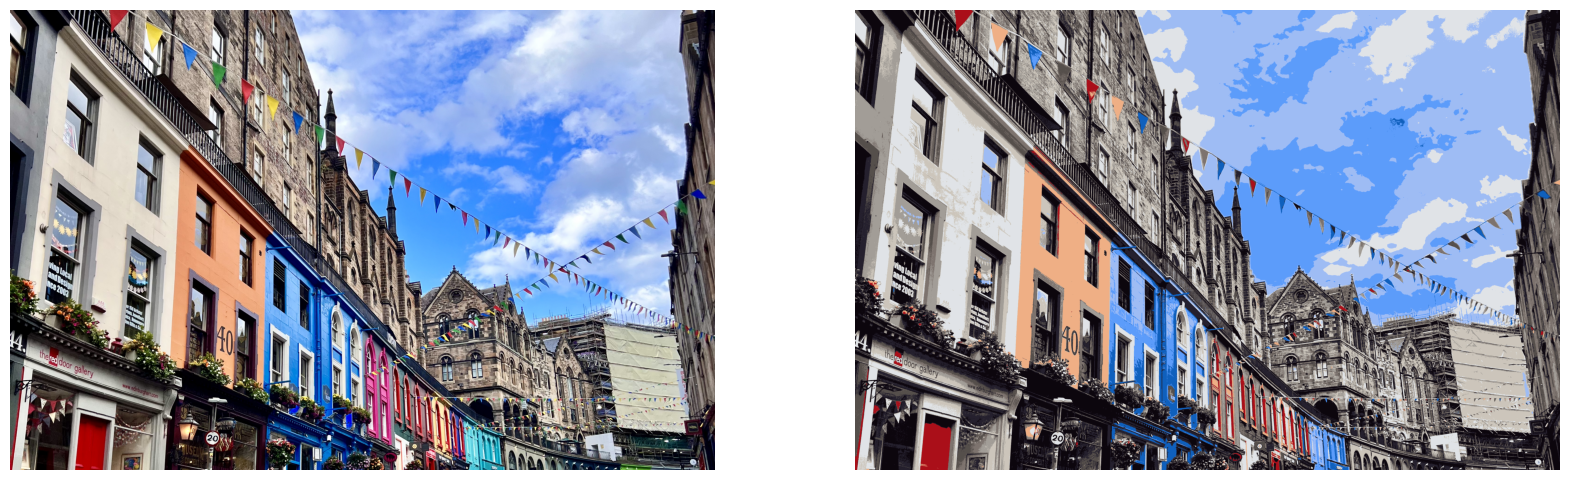
\includegraphics[width=0.9\linewidth]{Images/color_quantization.png}

    \caption{When a color is represented with too few bits, the transition between colors appears as discrete steps, known as color banding (right).}\label{fig:color-band}
\end{figure} 



Lastly, I would like to mention that the pixel-based displays discussed above is called raster graphics or raster displays. It lay outs the image onto a two-dimensional array of pixels with a grid of x and y coordinates on a display space. Here, zoom-in does not bring us any more details as we are limited by the image or screen resolution. To address this issue, vector graphics stores the shape of objects with mathematical expressions instead of pixel values. This offers flexibility with the resolution as the shape of the objects is computed based on the desired resolution.

\subsection{3D scene components}

A 3D scene is composed of objects of different sizes, shapes, and appearances . To render an image of a scene, we first need a viewpoint, which will be represented by a camera. This mimics the case in the human visual system (HVS) where we look at a scene from a certain viewpoint, and the image of the scene appears in our retina. Without any light, all scene components appear dark. Therefore, light is a crucial aspect while describing a scene. Another important aspect is geometry which describes the shape of the objects. Geometry, camera and light are three essential components of a 3D scene. While rendering a scene in a 3D software platform, such as Blender or Maya, a scene file contains all this information along with material/texture details. The light-material interaction defines the appearance, which this thesis is focused on. Before delving into the details of appearance, I will briefly review geometry as it builds up a baseline for the appearance representation in computer graphics.

\begin{figure}
  \centering
  % \fbox{\rule{0pt}{2in} \rule{0.9\linewidth}{0pt}}
   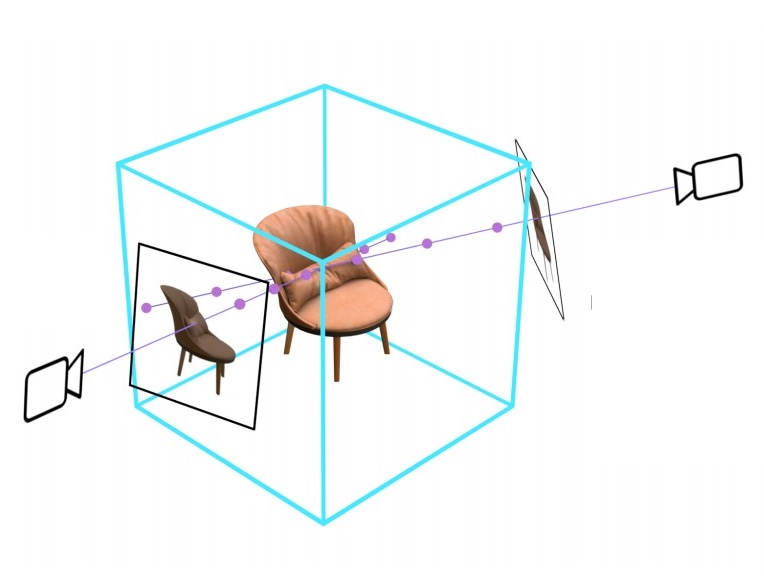
\includegraphics[width=0.7\linewidth]{Images/scene_with_camera.jpg}
   \caption{Rendering an image of a 3D scene requires lighting, viewpoint (camera) and geometry. Image courtesy of \citeauthor{boss2021nerd} \cite{boss2021nerd}.}
   \label{fig:teaser}
\end{figure}


\paragraph{Geometry.} In real world, what differentiates the state of the objects is the density of the matter the objects are made of. For instance, clouds are made of loosely connected molecules with large holes in-between. Wood and metal, on the other hand, are densely composed with little empty space between the molecules. On the other hand, computer graphics assumes that objects are either solid or not. This helps keep things simple since the external shape of an object is what matters at the end. 


In general, the shape of an object is represented with 3D points in computers' memory, with $x$, $y$, $z$ axes defined in the Cartesian coordinate system. The surface (a polygon) can then be constructed by connecting multiple points that lie on the same plane (co-planar). The simplest polygon we can create is a triangle. Triangles are widely used because of their simplicity and efficiency which led to the development of multiple efficient algorithms to compute the intersection of a triangle with a line. In case surfaces are defined by multiple points, it is common to  divide them into multiple triangles, known as triangulation. Although the real-world objects are not naturally polygonal, this simplification helps efficient rendering and digital representation.

\begin{figure}
  \centering
  % \fbox{\rule{0pt}{2in} \rule{0.9\linewidth}{0pt}}
   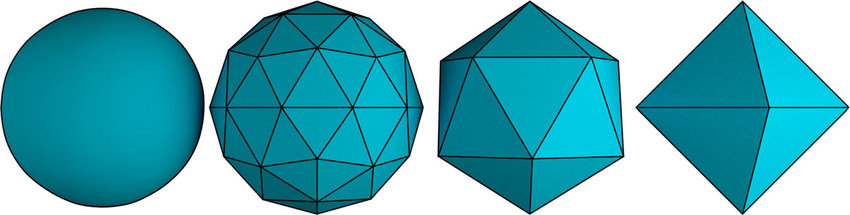
\includegraphics[width=0.7\linewidth]{Images/Triangulation-of-surfaces-Any-curved-surface-in-this-case-a-sphere-can-be-approximated.png}
   \caption{Triangulation of surfaces is a commonly used method in computer graphics to define surfaces. It allows the creation of complex shapes. Increasing the number of triangles also increases the resolution of the shape that leads to smoother surface representations. Image courtesy of \citeauthor{triangulation} \cite{triangulation}.}
   \label{fig:triangulation}
\end{figure}

One might wonder how triangulation handles the reconstruction of smooth surfaces. It is indeed not not optimal solution. However, considering a smooth curve, we can approximate it by taking a few points (samples) on the curve and connecting them with straight lines (segments). To enhance the resolution, we can take more samples, that is, reduce the size of the segments. Applying this to smooth surfaces, we can increase the number of triangles (Figure \ref{fig:triangulation}, which will eventually increase the rendering time. The process of converting a smooth surface to triangular mesh is known as tesselation.


Returning back to the early discussion on discretization, computer graphics only approximates the shape of the real-world continuous objects with discrete data. Since the ultimate goal is to display these shapes on a screen that also operates with discrete data, one well-known approach to conceal the triangular look of a surface is to keep the size of the triangles smaller than the pixel size. This approach has been used widely in both professional rendering programs, such Pixar's RenderMan, and recently taken its place in real-time applications.

Ray tracing algorithms, which HyperBRDF is built on, do not necessarily need a polygonal representation of objects. Ray tracing computes the intersection point of a ray (a straight line) with the object surface, which can be found either with a geometric or an algebraic solution. The algebraic solution becomes useful when the surfaces are defined by mathematical equations, known as implicit/algebraic surfaces. A ray equation, essentially a line equation, along with the mathematical equation for the surface of an object give us a system of linear equations, for which a solution exists if the ray and the object intersect.

 Although geometry can be defined by various methods, such as meshes, NURBS, subdivision surfaces, implicit surfaces, etc, this section only focuses on polygonal mesh representation. Triangle is the most common rendering primitive used in ray tracing and on modern GPUs. Since the support of only one primitive is preferred due to simplicity and efficiency, most 3D platforms first convert geometry to triangular meshes before rendering.
 
\subsection{Photo-realistic rendering}
There are different approaches to render an image of a scene. Whichever rendering method we choose, we should expect the same image as the output. In photo-realistic rendering, which is often the most desired, the expectation from a rendered image is to look the same as how our eyes perceive the scene. In other words, the image should look like a "photograph". Achieving such photo-realism requires us to understand two main aspects of our visual system: 1) geometric construction of the shapes with respect to other objects, 2) the physics laws behind appearance. More specifically, photo-realistic rendering focuses on simulating the behaviour of light throughout its propagation and its interaction with matter.

\paragraph{Perspective projection and visibility.}

The human visual system is inherently an optical system that converges light rays that are reflected from objects to a focal point. Following the geometry, our eyes perceive objects that are further away smaller than the closer objects of the same size. That is, objects get smaller in the rendered image in our retina as they move away from our eyes. This is known as foreshortening effect. The lens systems in cameras already replicate this effect, and photo-realistic rendering also aims to achieve this foreshortening effect along with simulating the physics laws for appearance.  

To achieve foreshortening effect, let us imagine we have a canvas or an image plane between the eye and the object. By tracing the lines from the eye to the corners of the objects, we can find the location of the projected corners (points) on the image plane. This is known as perspective projection. We can then draw the edges of the object on the image plane to complete the look. However, this look is unlikely to be photo-realistic as we haven't figured what edges are visible from the viewpoint. For instance, if it was an opaque cube, then the back sides would remain hidden behind the front sides. Therefore, rendering involves computations for the visibility problem along with the perspective projection. 

\begin{figure}[h]
  \centering
  % \fbox{\rule{0pt}{2in} \rule{0.9\linewidth}{0pt}}
   \includegraphics[width=0.6\linewidth]{Images/perspective_projection.png}
   \caption{}
   \label{fig:perspective_projection}
\end{figure}



There are different ways to project a 3D scene onto a flat surface. For instance, in artistic drawing, perspective projection can include multiple focal points (Figure \ref{fig:artistic_drawing}). However, computer graphics generally assumes one point of perspective as it mimics our visual system as well as cameras.  In this approach, the line of sight, the line from the eye perpendicular to the canvas, passes through the center of the canvas. Viewing frustum is then defined as the region of the scene that is projected onto the canvas. That is, the lines passing through the corners of the canvas comprise the corners of the frustum base. Here, we can change the size of the canvas, which results in the change of the frustum size, and so, the visible region of the scene. Akin to photography, changing the focal length of the camera lenses adjusts the field of view.

\begin{figure}[h]
  \centering
  % \fbox{\rule{0pt}{2in} \rule{0.9\linewidth}{0pt}}
   \includegraphics[width=0.4\linewidth, height=4.5cm]{Images/single_point_perspective.png}
    \includegraphics[width=0.4\linewidth, height=4.5cm]{Images/two_points_perspective.png}

   \caption{Single-point vs two-point perspective. Computer graphics mimics our visual system, focusing on single-point projection. However, multi-point perspective is widely explored in artistic drawing.}
   \label{fig:artistic_drawing}
\end{figure}


% \paragraph{Visibility problem}
The visibility problem occurs when some parts of the scene are not visible from a certain viewpoint. For instance, if we simply project the corners of an object and draw the edges, then some corners that shouldn't be visible from  a certain viewpoint will be included in the rendered image. Furthermore, some objects will be occluded by others, hiding them from the viewpoint. Computer graphics tackles the visibility problem in two different ways: rasterization, and ray tracing. I will not go into the details of these algorithms as this is beyond the focus of this thesis.

% In this section, I will mostly focus on ray tracing as HyperBRDF is designed for such renderers.Photo-realistic rendering aims to project or flatten a 3D scene onto an image plane that lies between the scene and the camera position or the viewpoint. Mimicking our visual system, we first apply perspective projection via similarity formula in geometry and then decide which points are visible from the viewpoint. Some will be indeed occluded by other objects or the front sides. 

\paragraph{Appearance.}
Perspective projection and visibility only projects the size and shape of the scene realistically without any consideration for appearance, such as the color, texture, brightness, etc. We can only perceive an object if the light bounces off its surface. Therefore, appearance is defined by the light-matter interactions, where the light travels in a ray form in space and gets absorbed or reflected when it interacts with the surface of an object. It can be emitted by different light sources, such as the sun, or light bulbs. After the light bounces off a surface, it continues its journey until it either reaches our eyes where it is converted to electrical signals or another surface where the interaction steps repeat.

The color of an object is defined by a mixture of the reflected light colors. The light color is a continuous spectrum with the visible light lying between 380 to 700 nanometers in wavelength. For instance, a leaf reflects green light, while absorbing the remaining visible spectrum. Another example would be a black object that absorbs all visible lights, or a white object that reflects them all.

\begin{wrapfigure}{l}{8.5cm}
  \centering
  % \fbox{\rule{0pt}{2in} \rule{0.9\linewidth}{0pt}}
   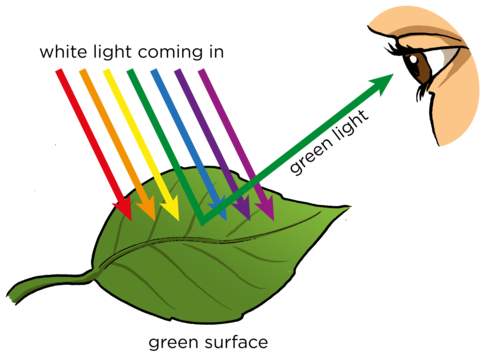
\includegraphics[width=0.5\linewidth]{Images/object-color.png}
   \caption{The reflected light from the surface of an object defines its color. \href{http://www.mstworkbooks.co.za/natural-sciences/gr8/images/gr8ec04-gd-0027.png}{Image source}}
   \label{fig:object-color}
\end{wrapfigure}



At the object level, reflection can be considered as a mirror-like look, where the light turns around the normal of the surface at the point of contact. The outgoing direction becomes the reflected version of the incoming one around this normal. Microscopic level interactions are more complex with light bouncing off in random directions, known as scattering. Computing the photon-atom interactions is indeed impractical. Therefore, computer graphics researchers have developed mathematical models to simulate the light-matter interactions at the microscopic level. I will discuss them later in this chapter. Section \ref{} will also compare HyperBRDF with such mathematical formulas. Here I will overview some of the well-known shading and lighting effects:

\textbf{\textit{Reflection}} occurs when light interacts with mirror-like objects that change the direction of light in the reverse direction with the same angle around the point of contact. The incoming light, also known as incident light, turns around the normal and leaves the surface in the reflected direction, outgoing direction (Figure \ref{fig:microfacet} - right). Metals, such as silver or aluminium are considered as materials with high reflectivity. Surface of the water or glass also creates reflection, but their reflectivity is considerably lower than metals.

\begin{wrapfigure}{r}{5.5cm}
\includegraphics[width=0.9\linewidth]{Images/rough_river_surface_reflection.png}
\caption{The ripples on the water's surface cause a blurred image of the bridge, acting as a rough surface.}\label{fig:water_reflection}
    
\end{wrapfigure} 

\textbf{\textit{Specular reflection}} appears when the surface is not perfectly smooth, and its roughness causes lights to bounce off in different directions. Imagine a rough surface at the microscopic level having many microfacets looking in slightly different directions. The complex nature of the material surface then reflects the lights at a microfacet level, each microfacet acting as a mirror (Figure \ref{fig:microfacet}). The overall outgoing light becomes the combination of each of these reflections, known as specular or glossy reflection. Most often, these microfacets are not visible to our eyes akin to smooth surface appearance. The deviation of lights from the mirror direction depends on how rough the surface is, that is, how varied the facet orientations are with respect to a smooth surface. More microfacets with higher variance in orientations will lead to greater divergence from the mirror angle, enlarging the glossy region of the surface. Here, roughness and glossiness are used antonymous to describe the specularity of a material. This type of reflection often leads to blurred or deformed image, as shown in Figure \ref{fig:water_reflection}. 



\begin{figure}
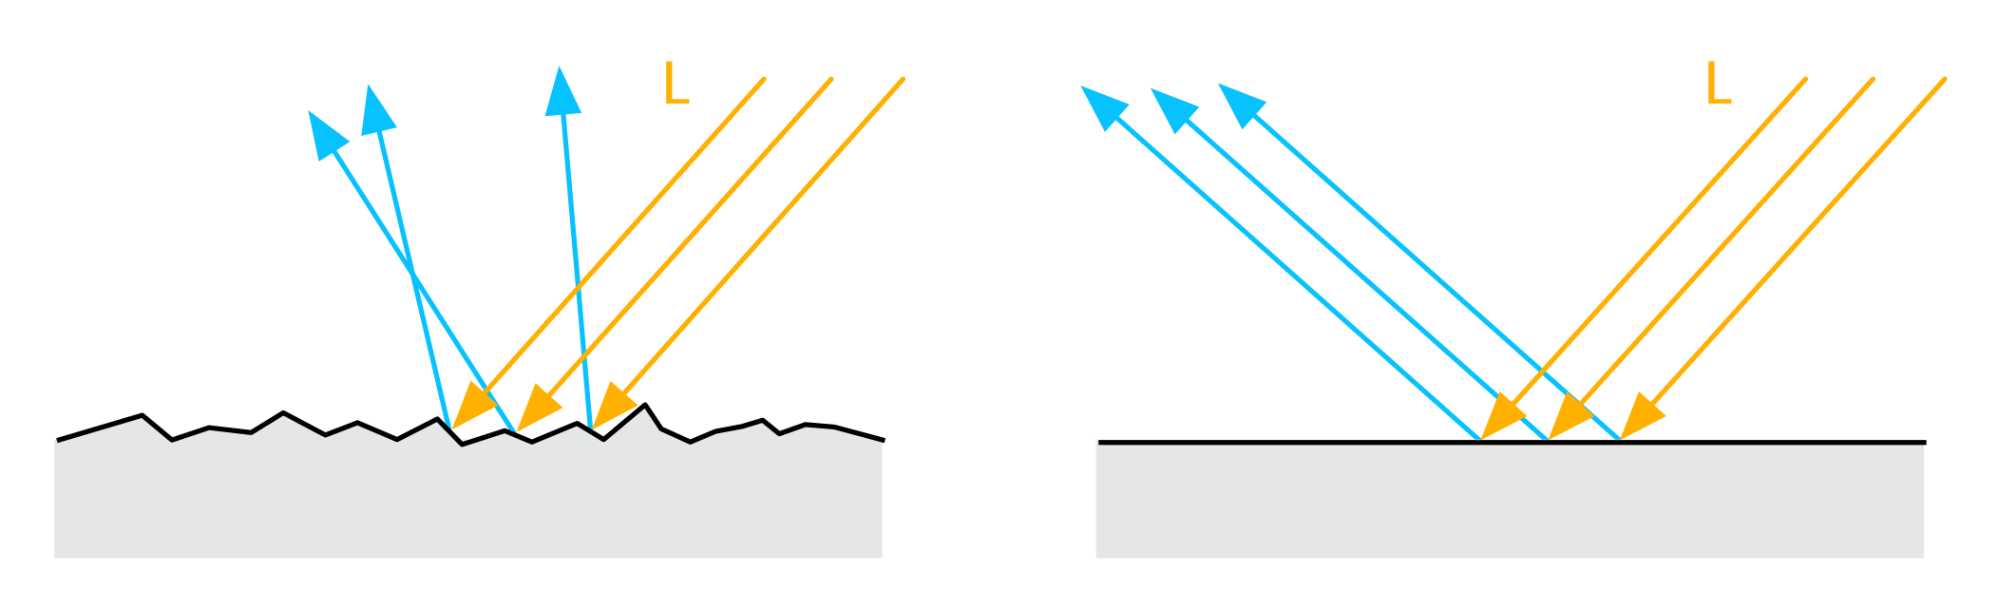
\includegraphics[width=0.9\linewidth]{Images/diagram_microfacet.png}
\caption{Reflection on a surface with microfacets vs smooth surface. Image from \citeauthor{googlePhysicallyBased} \cite{googlePhysicallyBased}}\label{fig:microfacet}
    
\end{figure} 


% \begin{figure}
%   \centering
%   % \fbox{\rule{0pt}{2in} \rule{0.9\linewidth}{0pt}}
%    \includegraphics[width=0.5\linewidth]{Images/rough_river_surface_reflection.png}
%    \caption{The ripples on the surface of the water causes a blurred image of the bridge, acting like a rough surface.}
%    \label{fig:water_reflection}
% \end{figure}


\textbf{\textit{Diffuse reflection}} is the reflection that we observe when the incident lights are so scattered that they reflect in random directions, equally spread. Diffuse surfaces are either extremely rough or composed of tiny structures where the light gets trapped, reflected and refracted multiple times before leaving the surface (Figure \ref{fig:diffuse-scattering}). The outgoing direction becomes independent from the incident direction due to the large number of internal reflection underneath the surface. This randomness results in the object appearing equally bright in all viewing directions. 

\begin{wrapfigure}{l}{6.5cm}
  \centering
  % \fbox{\rule{0pt}{2in} \rule{0.9\linewidth}{0pt}}
   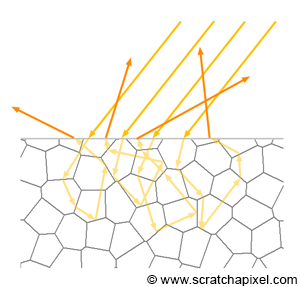
\includegraphics[width=0.5\linewidth]{Images/shad-diffuse1.png}
   \caption{Diffuse surfaces often have complex internal structures that cause the light to be reflected multiple times underneath the surface.}
   \label{fig:diffuse-scattering}
\end{wrapfigure}

Diffuse surfaces, also known as Lambertian or matte surfaces, differ from specular ones in that diffuse materials are often formed of multiple internal pieces that trap the light, causing the light's outgoing direction to become independent from the viewpoint. Specular ones, on the other hand, are modelled with microfacets that reflect the light rays around the mirror angle, remaining correlated with the incoming direction. As diffuse reflections are view-independent, the brightness of a diffuse surface remains consistent across all viewing angles. This distinction can be observed when looking at real-world materials, observing how their brightness changes when we move around, changing our viewpoint.


\begin{figure}[h]
  \centering
  % \fbox{\rule{0pt}{2in} \rule{0.9\linewidth}{0pt}}
   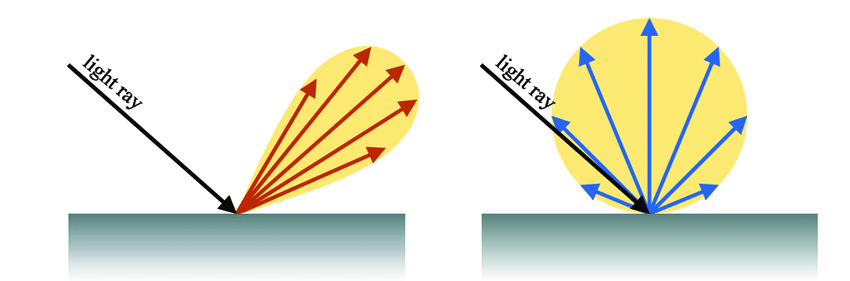
\includegraphics[width=0.7\linewidth]{Images/Differences-between-the-specular-and-diffuse-reflections-specuclar-reflections-occur-on.png}
   \caption{Specular vs diffuse reflection. Diffuse surfaces cause rays to scatter randomly, brightening the object equally in all viewing directions. Specular reflection is, on the other hand, view-dependent, reflected rays concentrated around the mirror reflection. Image courtesy of \citeauthor{specfig}.}
   \label{fig:specularvsdiffuse}
\end{figure}

Some other lighting and shading effects include transparency, subsurface scattering, indirect lighting and shadows. When light contacts a transparent object, such as glass or water, it bends and passes through the surface in a different direction, which can be computed using Snell's Law. Subsurface scattering, also known as translucency, occurs when light travels within the object, leaving the object at a different point and direction. Wax, marble or thin layers of skin are considered as translucent objects. Subsurface scattering is challenging to simulate. Indirect lighting is the result of the light being reflected from other surfaces, illuminating the object without any direct light from the light source. Lastly, shadows are dark regions due to blocked light by an object. 

The appearance of a scene depends on how light interacts with an object and the path light travels through. All the aforementioned effects contribute to appearance. Some effects, such as reflection, specularity, diffuse, transparency and subsurface scattering, relate to material properties. They affect shading, the appearance of an object. Other effects, shadows and indirect lighting, depend on the light's journey (light transport), that is, how much light the object gets after the light interacts with multiple surfaces. 

Shading is concerned with the interaction of light with the material. Light transport tracks the light's path throughout its journey while it bounces off surfaces. It takes into account the obstructions, changes of reflections, etc. In the real world, the two are not differentiated as they determine the appearance together. However, computer graphics keep these two distinct for efficient and practical computations. It is worth mentioning that simulating light-matter interactions is more challenging than tracking the light path. The latter is more straightforward, while the former requires simplifications for the material representations.



\paragraph{Ray tracing - Light transport simulation.}

Light starts its journey from a light source and travels in a straight line, bouncing off surfaces, Following this path is known as forward tracing. However, not all rays emitted from a source will reach the eye/camera. Considering their size, most rays are unlikely to contribute to our view of the scene, travelling in different directions. As it is highly impractical to trace all rays including those not contributing to our view, ray tracing algorithms trace the rays from the eye to the light source in the reverse direction for efficient computations (backward tracing).

The simulation starts with shooting rays from the virtual camera to the light source for each pixel on an image plane (Figure \ref{fig:raytracing}). Here, the view ray,  also known as primary or camera ray, passes through the center of a pixel on the image plane. The color of that pixel is computed by the shading algorithms that define the light-material interactions. Let's imagine we shoot a ray that encounters an object on its way to the light source. The intersection point can be computed by equating the mathematical equations defining the ray (a line) and the object. If a solution exists, then the object and the ray intersect. Once we obtain the intersection point with the object, we can shoot shadow rays from that point to the light source to calculate the diffuse and specular reflections at that point. If the shadow ray encounters another object before reaching the light source,  the intersection point remains in the shadow of the other object. Furthermore, the ray can be absorbed, reflected or refracted based on the material properties. In case of reflection, new rays can be spawned to compute the contribution of the reflection to the color of the object at that point.



\begin{figure}
  \centering
   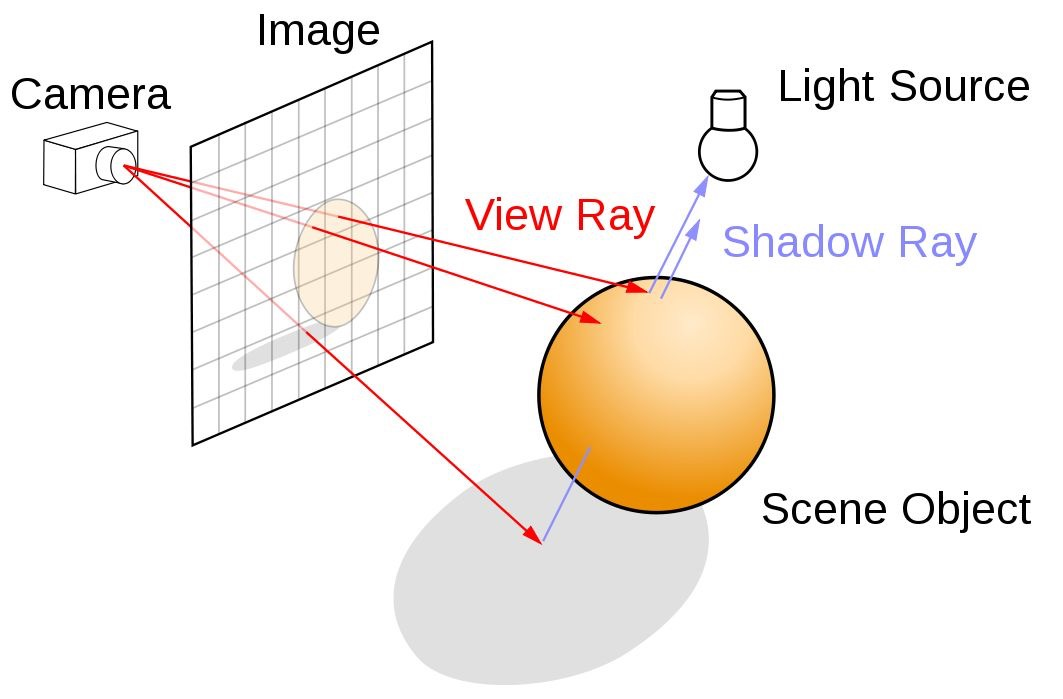
\includegraphics[width=0.5\linewidth]{Images/ray-tracing-image-1.jpg}
   \caption{Ray tracing simulate the light's journey to compute the color of each pixel on the rendered image. - Image courtesy of \href{https://commons.wikimedia.org/wiki/File:Ray_trace_diagram.svg}{Henrik, CC BY-SA 4.0}}
   \label{fig:raytracing}
\end{figure}

Shooting only one ray per pixel can cause artifacts, such as jagged edges or missing tiny objects. To alleviate such artifacts, we can shoot multiple rays in a sub-pixel grid or in a random setting. However, this increases the render time  because of the huge amount of computations required to trace the rays. This brings us to the trade-off between the render time and accuracy of the rendered image. This trade-off often leads to different applications, such as virtual effects in film industry requiring high accuracy with longer render time and real-time AR/VR applications with fast rendering but relatively low quality.

Ray tracing is a computationally-expensive rendering technique that simulates the light transport realistically, following the laws of physics. One important feature of ray tracing is that, it does not deal with perspective projection or visibility explicitly. Unlike rasterization, ray tracing inherently computes both by computing the intersection points of the ray with objects. Here, I explained the basics of the algorithm, which has been advanced in the recent years with intensive versions, known as path tracing. I will not go into the details of ray tracing as this thesis, more specifically HyperBRDF, is primarily focused on the shading part of the lighting simulations.

\subsection{Shaders and BRDF}

Shading is the process of computing the color of objects that are seen from the camera viewpoint. Earlier, we discussed that achieving photorealism involves two main steps:  visibility along with perspective projection and shading. If we are to achieve photorealism, then shading should reproduce the appearance of a scene so realistically that our eyes perceive the rendered image same as  the real word. A photorealistic image should look like a photograph of the same scene taken from the same viewpoint. 

Appearance is, in principle, the by-product of illumination and object properties. As the scene gets more light, objects are likely to appear brighter. Object properties that determine the appearance are reflectivity that defines light-material interactions and the geometric construction, i.e., orientation. The object color we perceive is the mixture of light rays reflected off the surface. Most often, objects do not emit light but lit by light sources emitting rays. This emitted light hits the surface of the object, some of which is later reflected off the surface and reaches our eyes, creating the color of the object. This type of lighting is known as direct lighting as the reflected light directly comes to our eyes after visiting the object. Indirect illumination occurs when an object gets some light reflected off other objects. Light can bounce off multiple surfaces, even infinitely many, before reaching our eyes.

Let's return to the discussion on lighting and shading effects we observe in the real world. We mentioned that what differentiates the objects with mirror-like,  specular and diffuse surfaces is the way they reflect the incoming light. A diffuse or Lambertian surface randomly spreads the incident light, looking equally bright in all viewing directions. Mirror-like objects reflect the ray around the point of contact, while specular surfaces distribute the light around the mirror direction. In the case of mirror-like or specular surfaces, the objects wouldn't be visible if our viewing direction is far from the mirror direction. Although we clearly distinguish different types of surfaces in computer graphics, real-world surfaces do not necessarily show only one kind of reflection.


Most real-world objects exhibit diffuse and specular reflections, having both components. This can happen because the object is composed of multiple materials with different reflectivities that are joined together, or it has multiple layers of materials that are added on top of each other as in the skin layers. Putting them together, we can define the overall appearance as the weighted sum of diffuse and specular components: $$I = k_d * I_d + k_s * I_s$$, where $I$ is the total intensity of the light reflected by the surface at the point of contact, $I_d$ and $I_s$  are diffuse and specular intensities, and $k_d$ and $k_s$ are their corresponding coefficients. Here, we oversimplify the equation for appearance, neglecting shadows and interaction between objects.



\begin{wrapfigure}{l}{7.5cm}
  \centering
  % \fbox{\rule{0pt}{2in} \rule{0.9\linewidth}{0pt}}
   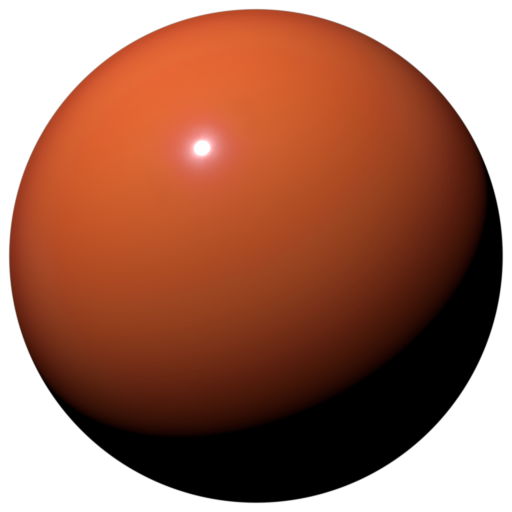
\includegraphics[width=0.5\linewidth]{Images/specular+diffuse.png}
   \caption{A material composed of both specular and diffuse components, lit by a point light source. The specular highlight (white circle) is centered around the light source direction. The material is specular-maroon-phenolic from MERL dataset \cite{Matusik2003jul}.}
   \label{fig:diffuse+spec}
\end{wrapfigure}


Here, we can compute the diffuse shading based on the angle between the normalized incident light direction $L$ and the normal to the surface $N$:
$$I_d = I_l \, k_d \cos(\theta) = I_l \, k_d \, (N . L)$$,  where $I_l$ is the intensity of the light source. Note that the lights with different colors can have different $I_l$ and $k_d$. Also, $\cos(\theta) < 0$ indicates that the light remains behind the surface, not contributing to the brightness on the visible side. The effect of $\cos$ term is visible in Figure \ref{fig:diffuse+spec}, where the diffuse intensity gets dimmer as the points on the surface gets further away from the point of contact (specular highlight). 

\begin{figure}[h]
  \centering
  % \fbox{\rule{0pt}{2in} \rule{0.9\linewidth}{0pt}}
   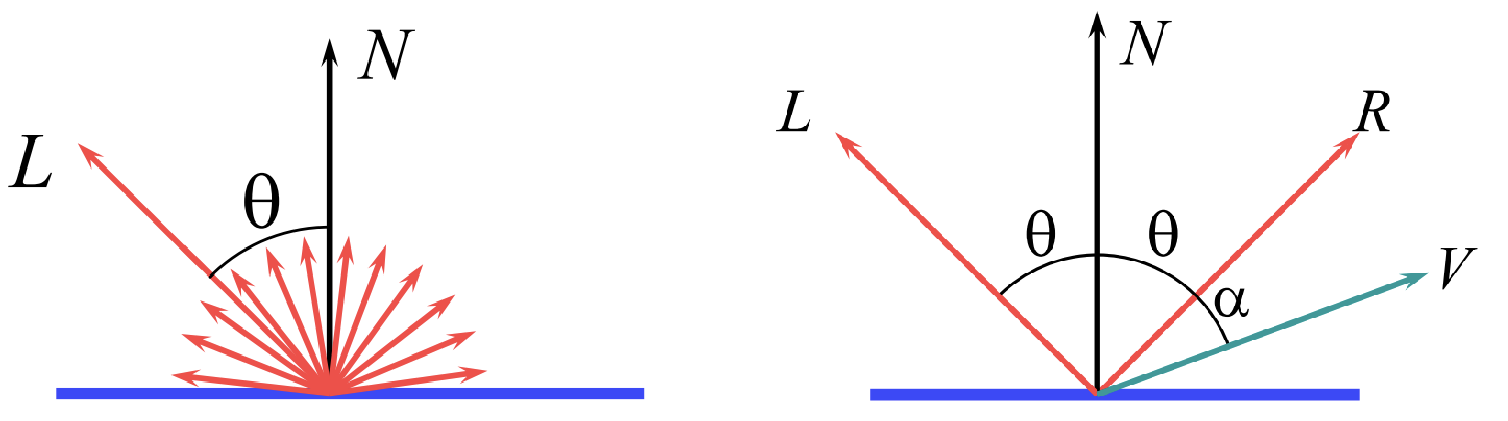
\includegraphics[width=0.5\linewidth]{Images/diffuse+specular+angle.pdf}
   \caption{Diffuse and specular reflections.. Figures from \href{https://www.cl.cam.ac.uk/teaching/2223/Graphics/Introduction_to_Graphics_1pp.pdf}{Slides by Rafal Mantiuk}}
   \label{fig:diffuse-spec-angle}
\end{figure}

The specular term can also be approximated by $$I_s = I_l \, k_s \, \cos^n(\alpha) = I_l \, k_s \, (R . V)^n $$, where $R$ is the mirror reflection, $V$ is the viewing direction, and $n$ is an ad-hoc roughness coefficient (Figure \ref{fig:diffuse-spec-angle}).


We mentioned that the consideration of only diffuse and specular reflections ignores indirect lighting, which can be compensated by adding a "cheat" constant term, $I_a * k_a$, known as ambient illumination. The overall shading then becomes:

\begin{equation}
I = I_a * k_a + \sum_i \, I_i \, k_d \, (N . L) + \sum_i \, I_i \, k_s \, (R_i . V)^n
\label{eq:Phong-eq}
\end{equation}

This mathematical model is known as Phong shading model, a well-known shading model used for decades in computer graphics. The simplified specular reflection term is introduced by Phong in 1998 \cite{phong1998illumination}. This model does not take into account the shadows, requiring ray tracing or  shadow mapping for shadows. It also considers the light sources to be infinitely far from the surface, ensuring the lighting direction $L$ remains same across the surface.

Modelling light-material interactions is very complex due to the nature of materials. Hence, computer graphics researchers have developed mathematical models to approximate the function defining the reflectance of a material surface. This function is known as Bidirectional Reflectance Distribution Function (BRDF). Phong shading model is one of the most popular BRDF approximation models due to its simplicity. Some other mathematical models include Cook-Torrance~\cite{cooktorrance1982}, Ward~\cite{ward1992} and GGX~\cite{walter2007microfacet}, with GGX being the most widely used approximation for its realistic results. I will compare HyperBRDF with GGX results in Chapter \ref{ch:HyperBRDF}.

Before going into the details of BRDF, let's examine the effect of the roughness term in the Phong model:

\begin{figure}[h]
  \centering
  % \fbox{\rule{0pt}{2in} \rule{0.9\linewidth}{0pt}}
   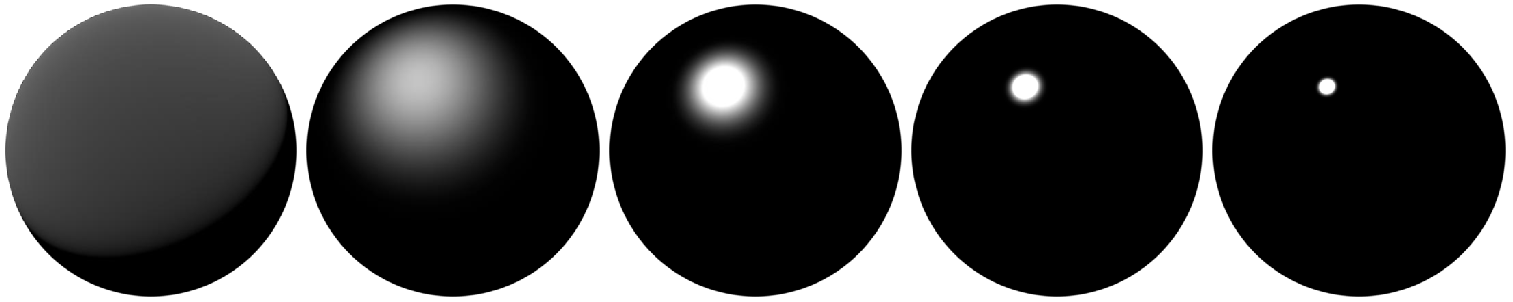
\includegraphics[width=\linewidth]{Images/Phong-roughness-coeff.pdf}
   \caption{Phong shading model implementation with decreasing roughness/increasing glossiness from left to right.}
   \label{fig:phong-roughness}
\end{figure}

The rougher the material surface is, the more matte the object appears. As we decrease its roughness by increasing the value $n$, the specular highlight becomes a mirror-like reflection around the point of contact. 


\paragraph{BRDF.} 
\begin{wrapfigure}{l}{7.5cm}
  \centering
  % \fbox{\rule{0pt}{2in} \rule{0.9\linewidth}{0pt}}
   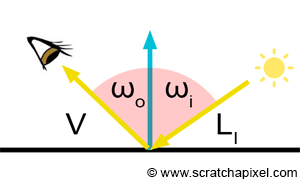
\includegraphics[width=\linewidth]{Images/shad2-brdfdir}
   \caption{BRDF depends on the incident light and viewing direction.}
   \label{fig:brdf}
\end{wrapfigure}
Looking at Eqn. \ref{eq:Phong-eq}, we observe that the appearance/shading depends on two variables, incoming light direction for diffuse and specular terms and viewing direction for specular only. Therefore, we can generalize this function with two parameters as  $f_R(\omega_o, \omega_i)$, where  $\omega_o$ is the angle between the surface normal and viewing direction and the surface normal and the light direction (Figure \ref{fig:brdf}). This function, known as as BRDF, gives us the amount of light reflected in the viewing direction when the surface is lit in the incoming light direction.

The mathematical formulations, such as Phong or GGX, approximate $BRDF(\omega_o, \omega_i)$s of real-world materials by making simplifying assumptions on their nature. For instance, some models are designed to simulate certain material types (Oren-Nayar model for Moon's BRDF). Some models follow the principle of optics or designed empirically (Phong). Fitting to measured BRDF values is another alternative approach, which recent neural network based models, including HyperBRDF, are built upon.  

Comparing the mathematical approximations to real-world measurements helps us understand how accurate the BRDF model represents a real-world material. $BRDF(\omega_o, \omega_i)$ itself is defined based on the laws of physics and can be physically measured by some specialised hardware, such as gonioreflectometer. Cameras can also be used to measure the BRDF. For instance, MERL dataset \cite{Matusik2003jul} is captured using a CCD camera. However, measuring the specular values can become a challenge with a camera capture due to the requirement of High Dynamic Range support. I will overview these capture systems in Chapter \ref{ch:HyperBRDF}.

The BRDF is essentially a radiometric term with the usage in computer graphics for realistic simulations of light-material interactions. Hence, physically-based BRDFs hold the following properties:
\begin{itemize}
  \item positivity $f_R(\omega_o, \omega_i) \geq 0$, BRDF is positive across valid incoming and outgoing directions.
  \item Helmholtz reciprocity: $f_R(\omega_o, \omega_i) = f_R(\omega_i, \omega_o)$, The surface acts the same if the incoming and outgoing directions are switched.
  \item energy conservation. Unless the object emits light, the reflected light cannot be larger than the received one.
\end{itemize}


Aiming for BRDF models to show these properties is essential to reproduce appearance realistically. In \citeauthor{Chenliang's paper} \cite{Chenliang's paper}, we discuss how to enforce the neural BRDF models to hold these properties. Rendering based on simulating the light's journey is computationally expensive. Therefore, a fast BRDF computation is another important factor while choosing a model. For instance, Phong is a simple model that requires fewer computations. However, it is not energy-conserving. Recent mathematical models, such as GGX, have replaced Phong due to more accurate representations. Nevertheless, mathematical models still oversimplify the complex real-world BRDFs, constrained with a few parameters to tune. Therefore, recent work has started developing neural network-based approaches, which can offer higher capacity for representations.

Lastly, we defined BRDF as the function of only two parameters, the incoming and outgoing directions. This brings us to the assumption that material properties remain the same across the whole surface. The complex real-world materials are composed of different substances, hence, they can reflect lights differently at different points of contact. This behaviour can be represented with a Spatially Varying Bidirectional Reflectance Distribution Function (SVBRDF) that has an additional location parameter ($f_R(\omega_o, \omega_i,  vec{x})$). Furthermore, we assume that the reflected light leaves the surface at the point of contact, which is unlikely the case for translucent materials where we observe subsurface  scattering. This behaviour can be represented with Bidirectional Surface Scattering Reflectance Distribution Function (BSSRDF) that has both entry and exit locations as additional parameters ($f_R(\omega_o, \vec{x_o}, \omega_i,  \vec{x_i})$). 

\subsection{Rendering Equation}

To conclude the rendering story, let's define the rendering equation that is being used to reproduce the appearance in ray tracing algorithms for the realistic simulation of light-material interactions.:
\begin{equation}
L_o(\vec{x}, \omega_o) = L_e(\vec{x}, \omega_o)  +  \int_S^2 L_i(\vec{x}, \omega_i) \, f_{\vec{x}}(\omega_o,  \omega_i) \, \abs{w_i . N} d\omega_i
\label{eqn:rendering-eqn}
\end{equation}
Here, $L_o(\vec{x}, \omega_o) $ is the outgoing light at point $x$ in the direction of $\omega_o$, $L_e(\vec{x}, \omega_o)$ is the emitted light that represents the light sources, $L_i(\vec{x}, \omega_i) $ is the incoming light at point $x$ in the direction of $\omega_i$, $f_{\vec{x}}(\omega_o,  \omega_i)$ is the BRDF, and $\abs{w_i . N} = \cos(\theta_i)$ is the Lambert's cosine term.

The rendering equation gives the outgoing light at point $x$ for a given incident light direction with the known BRDF. Here, we can define the BRDF term in multiple ways, such as with mathematical models discussed earlier, or a neural network outputting the BRDF value when fed with the directions, or physical measurements captured with special instruments. 

\section{Deep learning}
\subsection{Multilayer Perceptrons}
\subsection{Neural representations - Hypernetworks}
\subsection{Diffusion models}